% -*- latex -*-
%%%%%%%%%%%%%%%%%%%%%%%%%%%%%%%%%%%%%%%%%%%%%%%%%%%%%%%%%%%%%%%%
%%%%%%%%%%%%%%%%%%%%%%%%%%%%%%%%%%%%%%%%%%%%%%%%%%%%%%%%%%%%%%%%
%%%%
%%%% This text file is part of the source of 
%%%% `Parallel Programming in MPI and OpenMP'
%%%% by Victor Eijkhout, copyright 2012-2023
%%%%
%%%% mpi-morecollective.tex : obscure stuff
%%%%
%%%%%%%%%%%%%%%%%%%%%%%%%%%%%%%%%%%%%%%%%%%%%%%%%%%%%%%%%%%%%%%%
%%%%%%%%%%%%%%%%%%%%%%%%%%%%%%%%%%%%%%%%%%%%%%%%%%%%%%%%%%%%%%%%

\Level 0 {MPI Operators}
\label{sec:mpi-ops}
\index{operator|(}

MPI \emph{operators},
that is, objects of type \indexmpidef{MPI_Op},
are used in reduction operators.
Most common
operators, such as sum or maximum, have been built into the MPI
library; see section~\ref{sec:operator-list}.
It is also possible to define new operators; 
see section~\ref{sec:mpi-op-create}.

\Level 1 {Pre-defined operators}
\label{sec:operator-list}

The following is the list of \emph{pre-defined operators}\index{operator!predefined}
\indexmpishow{MPI_Op} values.

\input mpi-opstable

\Level 2 {Minloc and maxloc}
\label{sec:minmaxloc}

The \indexmpishow{MPI_MAXLOC} and \indexmpishow{MPI_MINLOC} operations
yield both the maximum and the rank on which it occurs. Their result
is a \lstinline{struct} of the data over which the reduction happens,
and an int. 

In C, the types to use in the reduction call are:
\indexmpidef{MPI_FLOAT_INT},
\indexmpidef{MPI_LONG_INT},
\indexmpidef{MPI_DOUBLE_INT},
\indexmpidef{MPI_SHORT_INT},
\indexmpidef{MPI_2INT},
\indexmpidef{MPI_LONG_DOUBLE_INT}.
Likewise, the input needs to consist of such structures:
the input should be an array of such struct types, where the \n{int} is
the rank of the number.

These types may have some unusual size properties:
%
\csnippetwithoutput{longintsize}{examples/mpi/c}{longint}

\begin{fortrannote}{Min/maxloc types}
  The original Fortran interface to MPI was designed around
  \fstandard{77} features,
  so it is not using Fortran derived types (\lstinline{Type} keyword).
  Instead, all integer indices are stored in whatever the type is that is
  being reduced. The available result types are then
  \indexmpidef{MPI_2REAL},
  \indexmpidef{MPI_2DOUBLE_PRECISION},
  \indexmpidef{MPI_2INTEGER}.

  Likewise, the input needs to be arrays of such type. Consider this example:
  \lstset{language=Fortran}
\begin{lstlisting}
Real*8,dimension(2,N) :: input,output
call MPI_Reduce( input,output, N, MPI_2DOUBLE_PRECISION, &
    MPI_MAXLOC, root, comm )
\end{lstlisting}
\end{fortrannote}

\begin{mplnote}{Operators}
  Arithmetic: \indexmplshow{plus}, \indexmplshow{multiplies}, \indexmplshow{max}, \indexmplshow{min}.

  Logic: \indexmplshow{logical_and}, \indexmplshow{logical_or}, \indexmplshow{logical_xor}.

  Bitwise: \indexmplshow{bit_and}, \indexmplshow{bit_or}, \indexmplshow{bit_xor}.
\end{mplnote}

\Level 1 {User-defined operators}
\label{sec:mpi-op-create}

In addition to predefined operators, MPI has the possibility of
\emph{user-defined operators}\index{operator!user-defined}
to use in a reduction or scan operation.

The routine for this is \indexmpiref{MPI_Op_create},
which takes a user function and turns it into
an object of type \indexmpishow{MPI_Op}, which can then be
used in any reduction:
%
\cverbatimsnippet[examples/mpi/c/reductpositive.c]{opcreatec}

\begin{pythonnote}{Define reduction operator}
  In python, \lstinline+Op.Create+ is a class method for the \lstinline+MPI+ class.
  %
  \pverbatimsnippet[examples/mpi/p/reductpositive.py]{opcreatep}
\end{pythonnote}

The user function needs to have the following signature:

\lstset{language=C}
\begin{lstlisting}
typedef void MPI_User_function
    ( void *invec, void *inoutvec, int *len, 
      MPI_Datatype *datatype); 
\end{lstlisting}

\lstset{language=Fortran}
\begin{lstlisting}
FUNCTION USER_FUNCTION( INVEC(*), INOUTVEC(*), LEN, TYPE) 
<type> INVEC(LEN), INOUTVEC(LEN) 
INTEGER LEN, TYPE 
\end{lstlisting}
\lstset{language=C}

For example, here is an operator for finding the smallest nonzero
number in an array of nonnegative integers:
%
\cverbatimsnippet[examples/mpi/c/reductpositive.c]{mpirwz}

\begin{pythonnote}{Reduction function}
  The python equivalent of such a function receives bare buffers as
  arguments. Therefore, it is best to turn them first into NumPy arrays
  using \indextermtt{np.frombuffer}:
  %
  \pverbatimsnippet[examples/mpi/p/reductpositive.py]{pmpirwz}
  %
  The \n{assert} statement accounts for the fact that this mapping of
  MPI datatype to NumPy dtype only works for built-in MPI datatypes.
\end{pythonnote}

\begin{mplnote}{User-defined operators}
  A user-defined operator can be a templated class with an \lstinline+operator()+.
  Example:
  \cxxverbatimsnippet{mpluserreduct}
  \cxxverbatimsnippet{mpluserreductuse}
  (The templated class can be a lambda expression)
\end{mplnote}

\begin{mplnote}{Lambda operator}
  You can also do the reduction by lambda:
  \cxxverbatimsnippet{mpllambdareduce}
\end{mplnote}

The function has an array length argument~\n{len}, to allow for
pointwise reduction on a whole array at once. The \n{inoutvec} array
contains partially reduced results, and is typically overwritten by
the function.

There are some restrictions on the user function:
\begin{itemize}
\item It may not call MPI functions, except for
  \indexmpishow{MPI_Abort}.
\item It must be associative; it can be optionally commutative, which
  fact is passed to the \indexmpishow{MPI_Op_create} call.
\end{itemize}

\begin{exercise}
  \label{ex:one-norm-op}
  Write the reduction function to implement the
  \emph{one-norm}\index{norm!one} of a vector:
  \[ \|x\|_1 \equiv \sum_i |x_i|. \]
  \skeleton{onenorm}
\end{exercise}

The operator can be destroyed with a corresponding
\indexmpidef{MPI_Op_free}.
\begin{lstlisting}
int MPI_Op_free(MPI_Op *op)
\end{lstlisting}
This sets the operator to \indexmpishow{MPI_OP_NULL}.
This is not necessary in \ac{OO} languages,
where the destructor takes care of it.

You can query the commutativity of an operator with
%
\indexmpiref{MPI_Op_commutative}.

\Level 1 {Local reduction}

The application of an \indexmpishow{MPI_Op} can be performed with the routine
\indexmpiref{MPI_Reduce_local}. Using this routine and some
send/receive scheme you can build your own global reductions. Note
that this routine does not take a communicator because it is purely local.

\index{operator|)}

\Level 0 {Nonblocking collectives}
\label{sec:mpi3collect}

Above you have seen how the `Isend' and `Irecv' routines can overlap communication
with computation. This is not possible with the collectives you have seen so far:
they act like blocking sends or receives.
However, there are also \indextermsub{nonblocking}{collectives},
introduced in \mpistandard{3}.

Such operations can be used to increase efficiency.
For instance, computing
\[ y \leftarrow Ax + (x^tx)y \]
involves a matrix-vector product, which is dominated by computation
in the \indextermsub{sparse}{matrix} case, and an inner product which is 
typically dominated by the communication cost. You would code this as
\begin{lstlisting}
MPI_Iallreduce( .... x ..., &request);
// compute the matrix vector product
MPI_Wait(request);
// do the addition
\end{lstlisting}

This can also be used for 3D FFT operations~\cite{Hoefler:case-for-nbc}.
Occasionally, a nonblocking collective can be used for nonobvious purposes,
such as the \indexmpishow{MPI_Ibarrier} in~\cite{Hoefler:2010:SCP}.

These have roughly the same calling sequence as their blocking counterparts,
except that they output an \indexmpishow{MPI_Request}. You
can then use an \indexmpishow{MPI_Wait} call to make sure the collective
has completed.

Nonblocking collectives offer a number of performance advantages:
\begin{itemize}
\item Do two reductions (on the same communicator) with different
  operators simultaneously:
\[ 
\begin{array}{l}
  \alpha\leftarrow x^ty\\
  \beta\leftarrow \|z\|_\infty
\end{array}
\]
which translates to:
\begin{lstlisting}
MPI_Allreduce( &local_xy,  &global_xy, 1,MPI_DOUBLE,MPI_SUM,comm);
MPI_Allreduce( &local_xinf,&global_xin,1,MPI_DOUBLE,MPI_MAX,comm);
\end{lstlisting}
\item do collectives on overlapping communicators simultaneously;
\item overlap a nonblocking collective with a blocking one.
\end{itemize}

\begin{exercise}
  \label{ex:procgridnonblock}
  Revisit exercise~\ref{ex:rowcolcomm}. Let only the first row and
  first column have certain data, which they broadcast through columns
  and rows respectively. Each process is now involved in two
  simultaneous collectives. Implement this with nonblocking
  broadcasts, and time the difference between a blocking and a
  nonblocking solution.
  \skeleton{procgridnonblock}
\end{exercise}

\begin{remark}
  Blocking and nonblocking don't match: either all processes
  call the nonblocking or all call the blocking one.
  Thus the following code is incorrect:
\begin{lstlisting}
if (rank==root)
  MPI_Reduce( &x /* ... */ root,comm );
else
  MPI_Ireduce( &x /* ... */ );
\end{lstlisting}
  This is unlike the point-to-point behavior of nonblocking calls:
  you can catch a message with \indexmpishow{MPI_Irecv}
  that was sent with \indexmpishow{MPI_Send}.
\end{remark}

\begin{remark}
  Unlike sends and received, collectives have no identifying tag.
  With blocking collectives that does not lead to ambiguity problems.
  With nonblocking collectives it means that all processes
  need to issue them in identical order.
\end{remark}

List of nonblocking collectives:
\begin{itemize}
\item 
  \indexmpidef{MPI_Igather},\indexmpidef{MPI_Igatherv},
  \indexmpiref{MPI_Iallgather},\indexmpidef{MPI_Iallgatherv},
\item 
  \indexmpidef{MPI_Iscatter}, \indexmpidef{MPI_Iscatterv},
\item 
  \indexmpidef{MPI_Ireduce},
  \indexmpiref{MPI_Iallreduce},
  \indexmpidef{MPI_Ireduce_scatter},
  \indexmpidef{MPI_Ireduce_scatter_block}.
\item 
  \indexmpidef{MPI_Ialltoall},\indexmpidef{MPI_Ialltoallv}, \indexmpidef{MPI_Ialltoallw},
\item 
  \indexmpishow{MPI_Ibarrier}; section~\ref{sec:ibarrier},
\item \indexmpidef{MPI_Ibcast},
\item \indexmpidef{MPI_Iexscan}, \indexmpidef{MPI_Iscan},
\end{itemize}

\begin{mplnote}{Nonblocking collectives}
  Nonblocking collectives have the same argument list as the
  corresponding blocking variant, except that
  instead of a \lstinline+void+ result,
  they return an \indexmplshow{irequest}.
  (See~\ref{mpl:irequest})

  Wait calls are methods of the \indexmplshow{irequest} object.
  %
  \cxxverbatimsnippet{mplireduce}
\end{mplnote}

\Level 1 {Examples}

\Level 2 {Array transpose}
\index{transpose|(}

To illustrate the overlapping of multiple nonblocking collectives,
consider transposing a data matrix.
Initially, each process has one row of the matrix;
after transposition each process has a column.
Since each row needs to be distributed to all processes,
algorithmically this corresponds to a series of scatter calls,
one originating from each process.
%
\cverbatimsnippet[examples/mpi/c/itransposeblock.c]{transposescatterref}
%
Introducing the nonblocking \indexmpishow{MPI_Iscatter} call,
this becomes:
%
\cverbatimsnippet[examples/mpi/c/itransposeblock.c]{itransposescatter}

\begin{exercise}
  Can you implement the same algorithm with \indexmpishow{MPI_Igather}?
\end{exercise}

\index{transpose|)}

\Level 2 {Stencils}

\begin{figure}[ht]
  \includegraphics[scale=.5]{graphcollective}
  \caption{Illustration of five-point stencil gather}
  \label{fig:5ptcollective}
\end{figure}

The ever-popular \indexterm{five-point stencil} evaluation
does not look like a collective operation, and indeed,
it is usually evaluated with (nonblocking) send/recv operations.
However, if we create a subcommunicator on each subdomain
that contains precisely that domain and its neighbors,
(see figure~\ref{fig:5ptcollective})
we can formulate the communication pattern as a gather on each of these.
With ordinary collectives this can not be formulated in a \indexterm{deadlock}-free
manner, but nonblocking collectives make this feasible.

We will see an even more elegant formulation of this operation
in section~\ref{sec:mpi-dist-graph}.

\Level 1 {Nonblocking barrier}
\label{sec:ibarrier}

Probably the most surprising nonblocking collective is the
\indextermsub{nonblocking}{barrier}
\indexmpiref{MPI_Ibarrier}. The way to understand this is to think of
a barrier not in terms of temporal synchronization, but state
agreement: reaching a barrier is a sign that a process has attained a
certain state, and leaving a barrier means that all processes are in
the same state. The ordinary barrier is then a blocking wait for
agreement, while with a nonblocking barrier:
\begin{itemize}
\item Posting the barrier means that a process has reached a certain
  state; and
\item the request being fullfilled means that all processes have
  reached the barrier.
\end{itemize}

One scenario would be \indexterm{local refinement}, where
some processes decide to refine their subdomain, which
fact they need to communicate to their neighbors.
The problem here is that most processes are not among these neighbors,
so they should not post a receive of any type.
Instead, any refining process sends to its neighbors,
and every process posts a barrier.

\cverbatimsnippet[examples/mpi/c/ibarrierprobe.c]{ibarrierpost}

Now every process alternately probes for messages
and tests for completion of the barrier.
Probing is done through the nonblocking \indexmpishow{MPI_Iprobe} call,
while testing completion of the barrier is done through
\indexmpishow{MPI_Test}.

\cverbatimsnippet[examples/mpi/c/ibarrierprobe.c]{ibarrierpoll}

We can use a nonblocking barrier to good effect, utilizing the idle
time that would result from a blocking barrier. In the following code
fragment processes test for completion of the barrier, and failing to
detect such completion, perform some local work.

\cverbatimsnippet[examples/mpi/c/findbarrier.c]{ibarrierwork}

\Level 0 {Performance of collectives}
\label{sec:collect-perform}

It is easy to visualize a broadcast as in figure~\ref{fig:bcast-simple}:
see figure~\ref{fig:bcast-simple}.
\begin{figure}[ht]
  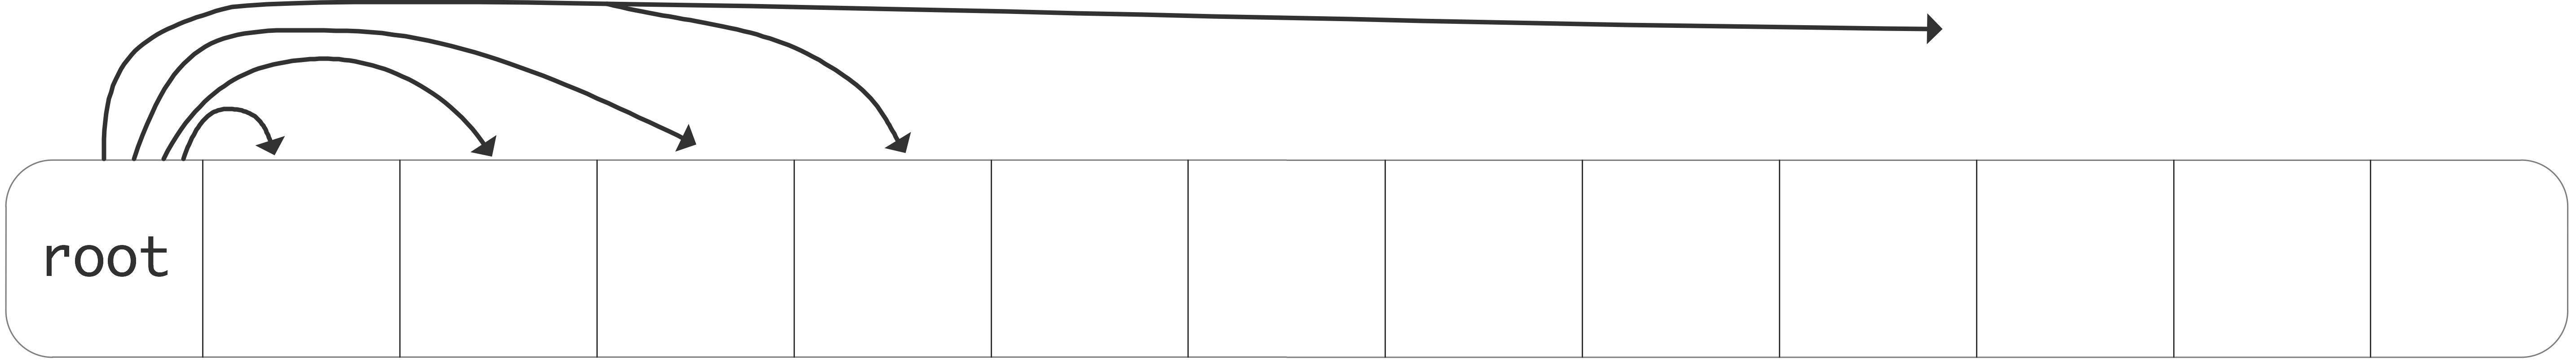
\includegraphics[scale=.08]{bcast-simple}
  \caption{A simple broadcast}
  \label{fig:bcast-simple}
\end{figure}
the root sends all of its data directly to every other process.
While this describes the semantics of the operation, in practice
the implementation works quite differently.

The time that a message takes can simply be modeled as
\[ \alpha +\beta n, \]
where $\alpha$~is the \indexterm{latency}, a~one time
delay from establishing the communication between two processes,
and $\beta$~is the time-per-byte, or the inverse of the \indexterm{bandwidth},
and $n$~the number of bytes sent.

Under the assumption that
a processor can only send one message at a time,
the broadcast in
figure~\ref{fig:bcast-simple} would take a time proportional to the
number of processors.

\begin{exercise}
  \label{ex:latencylinear}
  What is the total time required for a broadcast involving $p$
  processes?
  Give $\alpha$ and $\beta$ terms separately.
\end{exercise}

One way to ameliorate that is to structure the
broadcast in a tree-like fashion.
\begin{figure}[ht]
  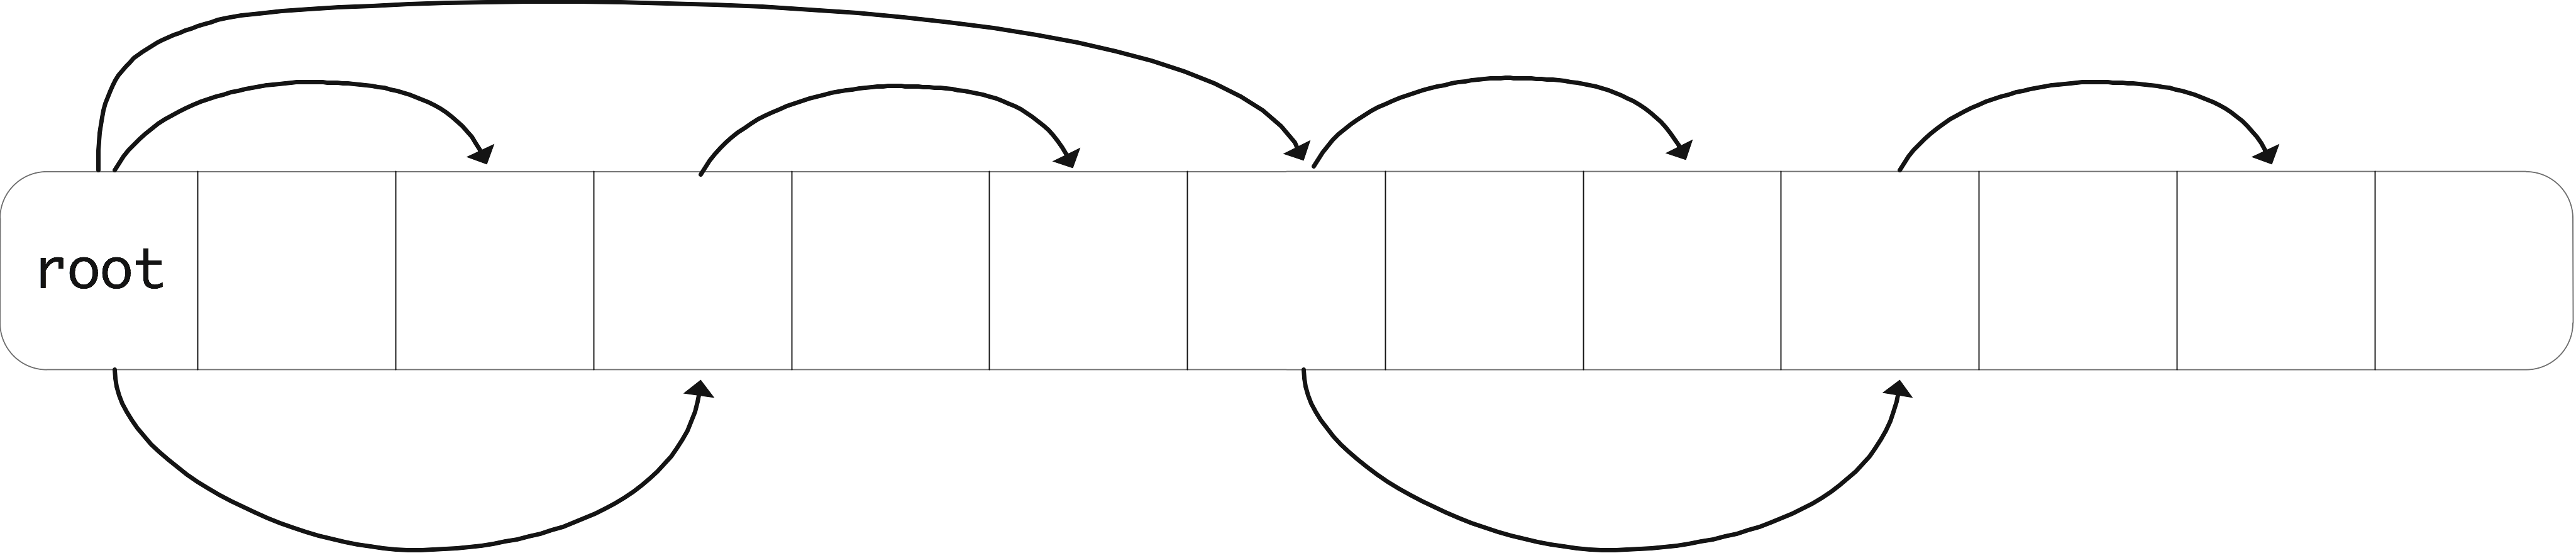
\includegraphics[scale=.1]{bcast-tree}
  \caption{A tree-based broadcast}
  \label{fig:bcast-tree}
\end{figure}
This is depicted in figure~\ref{fig:bcast-tree}.

\begin{exercise}
  \label{ex:latencylog}
  How does the
  communication time now depend on the number of processors, again
  $\alpha$ and $\beta$ terms separately.

  What would be a lower bound on the $\alpha,\beta$ terms?
\end{exercise}

The theory
of the complexity of collectives is described in more detail in
\HPSCref{sec:collective}; see also~\cite{Chan2007Collective}.

\Level 0 {Collectives and synchronization}
\label{sec:collect-sync}

Collectives, other than a barrier, have a synchronizing effect between processors.
For instance, in
\begin{lstlisting}
MPI_Bcast( ....data... root);
MPI_Send(....);
\end{lstlisting}
the send operations on all processors will occur after the root executes
the broadcast. 
\begin{figure}[ht]
  \includegraphics[scale=.35]{reduce-two-node}
  \caption{Trace of a reduction operation between two dual-socket 12-core nodes}
  \label{fig:trace-reduce}
\end{figure}
Conversely, in a reduce operation the root may have to wait for 
other processors. This is illustrated in figure~\ref{fig:trace-reduce}, which 
gives a TAU trace of
a reduction operation on two nodes, with two six-core sockets (processors) each.
We see that\footnote
{This uses mvapich version 1.6; in version 1.9 the implementation of an on-node reduction
has changed to simulate shared memory.}:
\begin{itemize}
\item In each socket, the reduction is a linear accumulation;
\item on each node, cores zero and six then combine their result;
\item after which the final accumulation is done through the network.
\end{itemize}
We also see that the two nodes are not perfectly in sync, which is normal for MPI
applications. As a result, core~0 on the first node will sit idle until it receives the partial
result from core~12, which is on the second node.

\begin{figure}[p]
  \footnotesize
  \leftskip=\unitindent
  \rightskip=\unitindent
The most logical execution is:\par\medskip

\includegraphics[scale=.35]{backintime1}

However, this ordering is allowed too:\par\medskip

\includegraphics[scale=.35]{backintime2}

Which looks from a distance like:\par\medskip

\includegraphics[scale=.35]{backintime3}

In other words, one of the messages seems to go `back in time'.

  \caption{Possible temporal orderings of send and collective calls}
  \label{fig:backintime}
\end{figure}

While collectives synchronize in a loose sense, it is not possible to
make any statements about events before and after the collectives
between processors:
\begin{lstlisting}
...event 1...
MPI_Bcast(....);
...event 2....
\end{lstlisting}
Consider a specific scenario:
\begin{lstlisting}
switch(rank) {
    case 0:
        MPI_Bcast(buf1, count, type, 0, comm);
        MPI_Send(buf2, count, type, 1, tag, comm);
        break;
    case 1:
        MPI_Recv(buf2, count, type, MPI_ANY_SOURCE, tag, comm, &status);
        MPI_Bcast(buf1, count, type, 0, comm);
        MPI_Recv(buf2, count, type, MPI_ANY_SOURCE, tag, comm, &status);
        break;
    case 2:
        MPI_Send(buf2, count, type, 1, tag, comm);
        MPI_Bcast(buf1, count, type, 0, comm);
        break;
}
\end{lstlisting}
Note the \indexmpishow{MPI_ANY_SOURCE} parameter in the receive calls on processor~1.
One obvious execution of this would be:
\begin{enumerate}
\item The send from~2 is caught by processor~1;
\item Everyone executes the broadcast;
\item The send from~0 is caught by processor~1.
\end{enumerate}
However, it is equally possible to have this execution:
\begin{enumerate}
\item Processor~0 starts its broadcast, then executes the send;
\item Processor~1's receive catches the data from~0, then it executes
  its part of the broadcast;
\item Processor~1 catches the data sent by~2, and finally processor~2
  does its part of the broadcast.
\end{enumerate}

This is illustrated in figure~\ref{fig:backintime}.
